
%(BEGIN_QUESTION)
% Copyright 2006, Tony R. Kuphaldt, released under the Creative Commons Attribution License (v 1.0)
% This means you may do almost anything with this work of mine, so long as you give me proper credit

Determine the LRV and URV points for a transmitter measuring water level in this vessel, with the $\Delta$P transmitter located 10 feet beneath the vessel and connected to it with capillary tubing and a remote seal filled with silicone fill fluid (SG = 0.934):

$$\includegraphics[width=15.5cm]{i00259x01.eps}$$

Be sure to show all your mathematical work so that your instructor will be able to check the conceptual validity of your technique(s).  A good way to check to see if you're solving the problem correctly is to check that each and every one of your intermediate calculations (i.e. the results you get mid-way during the process to arrive at the final answer) has real physical meaning.  {\bf If you truly understand what you are doing, you will be able to identify the correct unit of measurement for every intermediate result and also be able to show where that number applies to the scenario at hand}.

\vskip 20pt \vbox{\hrule \hbox{\strut \vrule{} {\bf Suggestions for Socratic discussion} \vrule} \hrule}

\begin{itemize}
\item{} Demonstrate how to {\it estimate} numerical answers for this problem without using a calculator.
\item{} When calculating hydrostatic pressures, there are two common methods: one is to use the formula $P = \gamma h$ and another is to translate inches of vertical liquid height directly into PSI using the known relationship between water and PSI (1 PSI = 27.68 inches of water).  Demonstrate both methods applied to this problem.
\item{} Identify some realistic situations that would justify the use of a remote seal on a pressure transmitter.
\item{} When using filled impulse lines (un-sealed), it is important to use a fill fluid denser than the fluid inside the process vessel.  Is this a requirement when using a remote (sealed) diaphragm?
\item{} Should the ``low'' side of the DP transmitter be vented or sealed?
\item{} What would happen if a technician inserted a pipe plug into the formerly open ``L'' port of the transmitter, sealing it off from atmospheric pressure?
\item{} What would happen if the capillary tube developed a leak?
\item{} Explain why this level transmitter does not require a {\it compensating leg}.
\end{itemize}

\underbar{file i00259}
%(END_QUESTION)





%(BEGIN_ANSWER)

%(END_ANSWER)





%(BEGIN_NOTES)

Calculating the hydrostatic pressure created by the 10 foot capillary tube (alone):

$$\left(10 \hbox{ ft silicone} \over 1 \right) \left(12 \hbox{ in} \over 1 \hbox{ ft} \right) \left(1 \hbox{ PSI} \over 27.68 \hbox{ in WC} \right) \left(0.934 \hbox{ in WC} \over 1 \hbox{ in silicone} \right) = 4.049 \hbox{ PSI}$$

\vskip 10pt

A full tank of water will add another 40 feet worth of hydrostatic pressure to the transmitter's ``H'' port:

$$\left(40 \hbox{ ft WC} \over 1 \right) \left(12 \hbox{ in} \over 1 \hbox{ ft} \right) \left(1 \hbox{ PSI} \over 27.68 \hbox{ in WC} \right) = 17.341 \hbox{ PSI}$$

\vskip 10pt

When the tank is empty (LRV condition), the transmitter only sees the 4.049 PSI created by the 10 feet of silicone fill fluid.  When the tank is full (URV condition), the transmitter sees the 4.049 PSI {\it plus} the 17.341 PSI created by the 40 feet of water, the total pressure being 21.390 PSI.

\vskip 10pt

LRV = 112.08 "W.C. = 4.049 PSI

\vskip 10pt

URV = 592.08 "W.C. = 21.390 PSI

%INDEX% Measurement, level: hydrostatic pressure (suppressed zero)

%(END_NOTES)


